% ================================================================
%  Script Matters: Measuring Latin-Script Banglish Robustness
%  in Bangla LLMs  —  B.Sc. Thesis Defense
%  Munim Thahmid (2005097) · Supervisor: Dr. Sadia Sharmin · BUET CSE
%  >>> Compile with: lualatex main.tex  (run twice)
% ================================================================
\documentclass[aspectratio=169,10pt]{beamer}

\usepackage{tikz}
\usetikzlibrary{arrows.meta,positioning,calc,shapes.geometric,backgrounds,fit,decorations.pathreplacing,shadows,fadings}
\usepackage{pgfplots}
\usepackage{booktabs}
\usepackage{array}
\usepackage{tcolorbox}
\tcbuselibrary{skins}
\usepackage{multirow}
\usepackage{pifont}
\usepackage{amssymb}
\usepackage{colortbl}

% ============================================================
%  Script Matters — custom clean beamer theme  (v2, visual)
%  Compile parent with lualatex (run twice for nav/refs)
% ============================================================

\usetheme{default}
\useinnertheme{rectangles}
\setbeamertemplate{navigation symbols}{}

% ---------- Fonts (lualatex + fontspec) ----------
\usepackage{fontspec}
\setsansfont{Noto Sans}[
  Renderer = HarfBuzz,
  UprightFont = *,
  BoldFont    = * Bold,
  ItalicFont  = * Italic,
  BoldItalicFont = * Bold Italic ]
\setmainfont{Noto Sans}[Renderer=HarfBuzz]
\setmonofont{DejaVu Sans Mono}[Scale=0.82]
\newfontfamily\bengalifont{Noto Sans Bengali}[
  Renderer = HarfBuzz,
  Script = Bengali,
  UprightFont = *,
  BoldFont = * Bold ]
\newcommand{\bn}[1]{{\bengalifont #1}}
\renewcommand{\familydefault}{\sfdefault}

% ---------- Colour palette ----------
\definecolor{buetnavy}{HTML}{16324F}    % deep header navy
\definecolor{buetnavy2}{HTML}{1B4068}
\definecolor{navytab}{HTML}{0F2538}      % darker strip for nav row
\definecolor{accent}{HTML}{2E78B5}       % section blue
\definecolor{accentlt}{HTML}{EDF5FC}     % pale blue panel
\definecolor{ink}{HTML}{23303B}          % body text
\definecolor{subink}{HTML}{5C6B78}       % muted text
\definecolor{rule}{HTML}{C9D6E2}
\definecolor{cardline}{HTML}{DCE4EC}
\definecolor{paper}{HTML}{F7F9FC}

% data-series colours (match thesis figures)
\definecolor{cBangla}{HTML}{2A9D8F}      % teal
\definecolor{cBanglish}{HTML}{E0734F}    % orange
\definecolor{cEnglish}{HTML}{3D6D8C}     % steel blue
\definecolor{good}{HTML}{2A9D8F}
\definecolor{bad}{HTML}{C24A3A}
\definecolor{warn}{HTML}{E0A33E}

% UI mock colours (for "Banglish in the wild")
\definecolor{msgblue}{HTML}{0A7CFF}      % outgoing chat bubble
\definecolor{msggray}{HTML}{E9E9EB}      % incoming chat bubble
\definecolor{ytred}{HTML}{FF0000}
\definecolor{starorange}{HTML}{F5A623}
\definecolor{uichrome}{HTML}{F1F3F4}

\setbeamercolor{normal text}{fg=ink}
\setbeamercolor{background canvas}{bg=paper}
\setbeamercolor{structure}{fg=accent}
\setbeamercolor{itemize item}{fg=accent}
\setbeamercolor{itemize subitem}{fg=cBanglish}
\setbeamercolor{alerted text}{fg=bad}
\setbeamercolor{frametitle}{fg=white,bg=buetnavy}

\setbeamerfont{frametitle}{series=\bfseries,size=\Large}
\setbeamerfont{title}{series=\bfseries,size=\huge}
\setbeamerfont{itemize/enumerate body}{size=\normalsize}
\setbeamerfont{itemize/enumerate subbody}{size=\small}

% ============================================================
%  Section navigation  (persistent top tabs, auto-tracked)
% ============================================================
\newcounter{secidx}\setcounter{secidx}{0}
\setbeamercolor{navbar}{bg=navytab,fg=white}

% one tab: #1 = its index, #2 = label
\newcommand{\navtab}[2]{%
  \ifnum\value{secidx}=#1\relax
    \tikz[baseline=-0.6ex]{\node[fill=accent,rounded corners=2.5pt,
       inner xsep=5pt,inner ysep=2pt,text=white,
       font=\bfseries\scriptsize]{#2};}%
  \else
    {\color{white!42}\scriptsize #2}%
  \fi}

\setbeamertemplate{headline}{%
  \nointerlineskip%
  \begin{beamercolorbox}[wd=\paperwidth,ht=2.3ex,dp=1.1ex,%
        leftskip=0.5cm,rightskip=0.5cm]{navbar}%
    \hbox to \dimexpr\paperwidth-1.0cm\relax{%
      \navtab{1}{Motivation}\hfil
      \navtab{2}{Benchmark}\hfil
      \navtab{3}{Results}\hfil
      \navtab{4}{Why It Fails}\hfil
      \navtab{5}{Frontier \& Scale}\hfil
      \navtab{6}{Mitigation}%
    }%
  \end{beamercolorbox}%
  \nointerlineskip\hbox{\color{accent}\rule{\paperwidth}{1.3pt}}%
}

% ---------- Frame title: navy bar with optional subtitle ----------
\setbeamertemplate{frametitle}{%
  \nointerlineskip%
  \begin{beamercolorbox}[wd=\paperwidth,ht=2.6ex,dp=1.4ex,leftskip=0.45cm,rightskip=0.45cm]{frametitle}%
    \insertframetitle\strut%
  \end{beamercolorbox}%
  \vskip0.30cm%
}
% helper for "Title | subtitle"
\newcommand{\subt}[1]{{\normalfont\fontsize{12}{12}\selectfont\;\textbf{|}\;#1}}

% ---------- itemize look ----------
\setbeamertemplate{itemize item}{\small\raise0.15ex\hbox{\textbullet}}
\setbeamertemplate{itemize subitem}{\scriptsize\raise0.2ex\hbox{--}}
\setlength{\leftmargini}{1.1em}

% ---------- Footline: name | short title | frame number ----------
\setbeamertemplate{footline}{%
  \hbox{%
    \begin{beamercolorbox}[wd=.36\paperwidth,ht=2.6ex,dp=1.1ex,leftskip=.3cm]{}%
      {\color{subink}\scriptsize Munim Thahmid \textbullet\ 2005097}%
    \end{beamercolorbox}%
    \begin{beamercolorbox}[wd=.40\paperwidth,ht=2.6ex,dp=1.1ex,center]{}%
      {\color{subink}\scriptsize Script Matters}%
    \end{beamercolorbox}%
    \begin{beamercolorbox}[wd=.24\paperwidth,ht=2.6ex,dp=1.1ex,rightskip=.3cm]{}%
      \hfill{\color{subink}\scriptsize\insertframenumber\,/\,\inserttotalframenumber}%
    \end{beamercolorbox}%
  }%
}

% ============================================================
%  BUET logo badge (red gear on a white disc → works on navy)
% ============================================================
\newcommand{\buetbadge}[1]{% #1 = diameter, e.g. 1.1cm
  \tikz{\node[circle,fill=white,inner sep=1.4pt,line width=0pt]
        {
\includegraphics[width=#1]{buetlogo.png}};}}

% ---------- Section divider frames (auto-numbered) ----------
\tikzfading[name=divfade,left color=transparent!0,right color=transparent!100]
\newcommand{\sectiondivider}[2]{%
  \stepcounter{secidx}%
  {\setbeamertemplate{footline}{}%
  \begin{frame}[plain]
    \begin{tikzpicture}[remember picture,overlay]
      \fill[buetnavy] (current page.south west) rectangle (current page.north east);
      % dissolving-script artwork, right side, faded into the navy
      \node[anchor=east,inner sep=0pt] (art) at (current page.east)
        {
\includegraphics[height=\paperheight]{img/script-dissolve.png}};
      \fill[buetnavy,path fading=divfade]
        (art.north west) rectangle ([xshift=3.0cm]art.south west);
      \fill[accent] ([yshift=-0.9cm]current page.west)
        rectangle ([xshift=-6.1cm,yshift=-1.5cm]current page.east);
      \node[anchor=west,text=accentlt,font=\bfseries\footnotesize]
        at ([xshift=1.0cm,yshift=2.05cm]current page.west)
        {SECTION \thesecidx\, /\, 6};
      % progress dots
      \coordinate (dotbase) at ([xshift=4.2cm,yshift=2.05cm]current page.west);
      \foreach \i in {1,...,6}{%
        \ifnum\i=\value{secidx}
          \fill[accent] ($(dotbase)+(\i*0.34cm,0)$) circle (0.075);
        \else
          \fill[white!25] ($(dotbase)+(\i*0.34cm,0)$) circle (0.05);
        \fi}
      \node[anchor=west,text=white,font=\bfseries\fontsize{28}{32}\selectfont,text width=8.8cm]
        at ([xshift=1.0cm,yshift=0.9cm]current page.west) {#1};
      \node[anchor=west,text=accentlt,font=\large,text width=8.6cm]
        at ([xshift=1.05cm,yshift=-2.15cm]current page.west) {#2};
      \node[anchor=south west,text=white!55,font=\scriptsize]
        at ([xshift=1.0cm,yshift=0.7cm]current page.south west) {Script Matters \textbullet\ BUET CSE};
      \node[anchor=south east] at ([xshift=-1.0cm,yshift=0.65cm]current page.south east)
        {\buetbadge{1.0cm}};
    \end{tikzpicture}
  \end{frame}}
}

% ============================================================
%  Handy boxes
% ============================================================
\newtcolorbox{keybox}{
  colback=accentlt, colframe=accent, boxrule=0.8pt, arc=2pt,
  left=8pt,right=8pt,top=6pt,bottom=6pt, enhanced,
  borderline west={3pt}{0pt}{accent},
  before upper={\raggedright\setlength{\parindent}{0pt}}
}
\newtcolorbox{takebox}[1]{
  colback=cBangla!8, colframe=cBangla, boxrule=0.8pt, arc=2pt,
  left=8pt,right=8pt,top=5pt,bottom=5pt, enhanced,
  fonttitle=\bfseries\color{white}, coltitle=white,
  colbacktitle=cBangla, title={#1},
  before upper={\raggedright\setlength{\parindent}{0pt}}
}

% ---------- Stat card: big coloured number + caption ----------
% \statcard{width}{accentcolour}{BIGNUMBER}{caption}
\newcommand{\statcard}[4]{%
  \begin{tcolorbox}[width=#1,colback=white,colframe=cardline,boxrule=0.6pt,
     arc=3pt,left=7pt,right=5pt,top=4pt,bottom=4pt,enhanced,nobeforeafter,
     borderline west={3pt}{0pt}{#2},drop fuzzy shadow={cardline}]
    {\color{#2}\bfseries\fontsize{20}{21}\selectfont #3}\\[1.5pt]
    {\color{subink}\scriptsize #4}
  \end{tcolorbox}}

% ---------- Plain feature card (icon + title + body) ----------
% \featurecard{width}{accentcolour}{\icon}{title}{body}
\newcommand{\featurecard}[5]{%
  \begin{tcolorbox}[width=#1,colback=white,colframe=cardline,boxrule=0.6pt,
     arc=3pt,left=7pt,right=7pt,top=4pt,bottom=4pt,enhanced,nobeforeafter,
     borderline west={3pt}{0pt}{#2},drop fuzzy shadow={cardline}]
    {\color{#2}#3\ \bfseries\footnotesize #4}\\[2pt]
    {\color{ink}\scriptsize #5}
  \end{tcolorbox}}

% chips
\newcommand{\chip}[2]{\tikz[baseline=(x.base)]{\node[fill=#1,rounded corners=2pt,inner sep=2.5pt,text=white,font=\footnotesize\bfseries](x){#2};}}

% model-name pill (light, for protocol slide)
\newcommand{\mchip}[1]{\tikz[baseline=(x.base)]{\node[fill=accentlt,draw=rule,line width=0.5pt,
  rounded corners=3.5pt,inner xsep=5pt,inner ysep=3pt,text=ink,font=\scriptsize\bfseries](x){#1};}}

% inline data bar for result tables: \accbar{count}{max}{colour}
\newcommand{\accbar}[3]{%
  \tikz[baseline=-0.35ex]{%
    \fill[#3!16] (0,0) rectangle (1.25,0.15);
    \fill[#3]    (0,0) rectangle ({1.25*#1/#2},0.15);}\,%
  {\footnotesize #1}}

% ============================================================
%  Lightweight TikZ line-icons  ( \ic{name}{colour} )
% ============================================================
\tikzset{
  icbase/.style={line width=1.0pt,line cap=round,line join=round}
}
% each icon drawn inside a 1em-ish box, baseline aligned
\newcommand{\ic}[2]{% #1 = name, #2 = colour
  \tikz[baseline=-0.55ex,scale=0.95]{\csname icon@#1\endcsname{#2}}}

\makeatletter
\newcommand{\icon@chat}[1]{% speech bubble
  \draw[icbase,#1] (0,0.05) -- (0,0.18)
    .. controls (0,0.30) and (0.10,0.36) .. (0.22,0.36)
    -- (0.46,0.36)
    .. controls (0.58,0.36) and (0.68,0.30) .. (0.68,0.18)
    -- (0.68,0.06)
    .. controls (0.68,-0.06) and (0.58,-0.12) .. (0.46,-0.12)
    -- (0.20,-0.12) -- (0.10,-0.24) -- (0.10,-0.12)
    .. controls (0.03,-0.12) and (0,-0.04) .. (0,0.05) -- cycle;}
\newcommand{\icon@search}[1]{% magnifier
  \draw[icbase,#1] (0.10,0.34) circle (0.16);
  \draw[icbase,#1] (0.22,0.10) -- (0.38,-0.06);}
\newcommand{\icon@star}[1]{\node[#1]{\ding{72}};}
\newcommand{\icon@check}[1]{\draw[icbase,#1] (0,0.06) -- (0.14,-0.10) -- (0.44,0.30);}
\newcommand{\icon@cross}[1]{\draw[icbase,#1] (0.02,0.30) -- (0.40,-0.10);
  \draw[icbase,#1] (0.40,0.30) -- (0.02,-0.10);}
\newcommand{\icon@warn}[1]{% warning triangle
  \draw[icbase,#1] (0.22,0.40) -- (0.46,-0.10) -- (-0.02,-0.10) -- cycle;
  \draw[icbase,#1] (0.22,0.26) -- (0.22,0.08);
  \fill[#1] (0.22,-0.01) circle (0.025);}
\newcommand{\icon@flask}[1]{% science flask
  \draw[icbase,#1] (0.10,0.36) -- (0.10,0.14) -- (-0.04,-0.10)
    .. controls (-0.08,-0.16) and (-0.02,-0.20) .. (0.06,-0.20)
    -- (0.40,-0.20)
    .. controls (0.48,-0.20) and (0.54,-0.16) .. (0.50,-0.10)
    -- (0.36,0.14) -- (0.36,0.36);
  \draw[icbase,#1] (0.04,0.36) -- (0.42,0.36);
  \draw[icbase,#1] (0.02,0.02) -- (0.44,0.02);}
\newcommand{\icon@target}[1]{% target / paired
  \draw[icbase,#1] (0.22,0.12) circle (0.24);
  \draw[icbase,#1] (0.22,0.12) circle (0.11);
  \fill[#1] (0.22,0.12) circle (0.03);}
\newcommand{\icon@scale}[1]{% balance / boundary
  \draw[icbase,#1] (0.22,0.40) -- (0.22,-0.16);
  \draw[icbase,#1] (-0.02,0.30) -- (0.46,0.30);
  \draw[icbase,#1] (0.06,-0.16) -- (0.38,-0.16);
  \draw[icbase,#1] (-0.02,0.30) .. controls (-0.10,0.10) and (0.06,0.10) .. (-0.02,0.30);
  \draw[icbase,#1] (-0.10,0.12) -- (0.06,0.12);
  \draw[icbase,#1] (0.38,0.12) -- (0.54,0.12);}
\newcommand{\icon@ruler}[1]{% tokens / measurement
  \draw[icbase,#1] (-0.02,0.30) rectangle (0.46,0.04);
  \foreach \x in {0.08,0.16,0.24,0.32,0.40}
    \draw[icbase,#1] (\x,0.30) -- (\x,0.18);}
\newcommand{\icon@gear}[1]{% mitigation / fix
  \draw[icbase,#1] (0.22,0.12) circle (0.13);
  \foreach \a in {0,45,...,315}
    \draw[icbase,#1] (\a:0.13)++(0.22,0.12) -- ++(\a:0.09);}
\newcommand{\icon@bolt}[1]{% gap / shock
  \draw[icbase,#1,fill=#1] (0.26,0.40) -- (0.06,0.10) -- (0.20,0.10)
     -- (0.14,-0.18) -- (0.40,0.16) -- (0.24,0.16) -- cycle;}
\newcommand{\icon@doc}[1]{% reviewed doc
  \draw[icbase,#1] (0.04,0.38) -- (0.04,-0.16) -- (0.42,-0.16) -- (0.42,0.24)
     -- (0.28,0.38) -- cycle;
  \draw[icbase,#1] (0.28,0.38) -- (0.28,0.24) -- (0.42,0.24);
  \draw[icbase,#1] (0.12,0.06) -- (0.34,0.06);
  \draw[icbase,#1] (0.12,-0.04) -- (0.34,-0.04);}
\newcommand{\icon@globe}[1]{% language / script
  \draw[icbase,#1] (0.22,0.12) circle (0.24);
  \draw[icbase,#1] (-0.02,0.12) -- (0.46,0.12);
  \draw[icbase,#1] (0.22,0.36) .. controls (0.04,0.24) and (0.04,0.0) .. (0.22,-0.12);
  \draw[icbase,#1] (0.22,0.36) .. controls (0.40,0.24) and (0.40,0.0) .. (0.22,-0.12);}
\makeatother

% ---------- table state markers (capability matrix) ----------
\newcommand{\cyes}{\ic{check}{good}}
\newcommand{\cno}{\ic{cross}{subink!55}}
\newcommand{\cpart}{\tikz[baseline=-0.5ex]{%
  \fill[warn] (0,0) -- ++(0,0.10) arc (90:270:0.10) -- cycle;
  \draw[warn,line width=0.7pt] (0,0) circle (0.10);}}

% ============================================================
%  pgfplots defaults
% ============================================================
\pgfplotsset{compat=1.18}
\pgfplotsset{
  every axis/.append style={
    font=\footnotesize,
    axis line style={rule},
    tick label style={color=ink},
    label style={color=ink},
    title style={color=ink,font=\small\bfseries},
    grid style={rule!60,line width=0.3pt},
  }
}


\title{Script Matters}
\subtitle{Measuring Latin-Script Banglish Robustness in Bangla LLMs}
\author{Munim Thahmid}
\date{June 2026}

% ---- column helpers
\newcolumntype{L}[1]{>{\raggedright\arraybackslash}p{#1}}
\newcolumntype{C}[1]{>{\centering\arraybackslash}p{#1}}
\newcommand{\gp}[1]{\textbf{\color{bad}#1}}     % negative gap
\newcommand{\gpp}[1]{\textbf{\color{good}#1}}    % positive gap

\begin{document}

% =====================================================  1. TITLE
{\setbeamertemplate{footline}{}
\begin{frame}[plain]
\begin{tikzpicture}[remember picture,overlay]
  \fill[buetnavy] (current page.south west) rectangle (current page.north east);

  % thin accent frame, top and bottom edges
  \fill[accent] (current page.north west) rectangle ([yshift=-0.13cm]current page.north east);
  \fill[accent] (current page.south west) rectangle ([yshift=0.13cm]current page.south east);

  % faint script-morph bookends in free corners
  \node[anchor=center,text=white!6!buetnavy,font=\fontsize{95}{95}\selectfont\bengalifont\bfseries]
     at ([xshift=1.9cm,yshift=1.6cm]current page.south west) {\bn{অ}};
  \node[anchor=center,text=white!6!buetnavy,font=\bfseries\itshape\fontsize{95}{95}\selectfont]
     at ([xshift=-1.8cm,yshift=-1.7cm]current page.north east) {a};

  % institutional header, centered
  \node[anchor=north] at ([yshift=-0.42cm]current page.north) {\buetbadge{0.92cm}};
  \node[anchor=north,text=white!92,font=\footnotesize\bfseries]
     at ([yshift=-2.18cm]current page.north)
     {BANGLADESH UNIVERSITY OF ENGINEERING AND TECHNOLOGY};
  \node[anchor=north,text=white!62,font=\scriptsize]
     at ([yshift=-2.65cm]current page.north)
     {Department of Computer Science and Engineering};

  % title block, centered
  \fill[accent] ([xshift=-1.4cm,yshift=1.28cm]current page.center)
     rectangle ([xshift=1.4cm,yshift=1.35cm]current page.center);
  \node[anchor=center,text=white,font=\bfseries\fontsize{40}{42}\selectfont]
     at ([yshift=0.42cm]current page.center) {Script Matters};
  \node[anchor=center,text=accentlt,font=\fontsize{14}{18}\selectfont]
     at ([yshift=-0.65cm]current page.center)
     {Measuring Latin-Script \textbf{Banglish Robustness} in Bangla LLMs};

  % presenter & supervisor, side by side
  \coordinate (prow) at ([yshift=2.05cm]current page.south);
  \node[anchor=center,text=accent!45!white,font=\tiny\bfseries]
     at ([xshift=-3.6cm,yshift=0.55cm]prow) {PRESENTED BY};
  \node[anchor=center,text=white,font=\large\bfseries]
     at ([xshift=-3.6cm]prow) {Munim Thahmid};
  \node[anchor=center,text=white!65,font=\footnotesize]
     at ([xshift=-3.6cm,yshift=-0.5cm]prow) {Student ID 2005097};
  \draw[white!25,line width=0.6pt]
     ([yshift=0.7cm]prow) -- ([yshift=-0.6cm]prow);
  \node[anchor=center,text=accent!45!white,font=\tiny\bfseries]
     at ([xshift=3.6cm,yshift=0.55cm]prow) {SUPERVISED BY};
  \node[anchor=center,text=white,font=\large\bfseries]
     at ([xshift=3.6cm]prow) {Dr.\ Sadia Sharmin};
  \node[anchor=center,text=white!65,font=\footnotesize]
     at ([xshift=3.6cm,yshift=-0.5cm]prow) {Department of CSE, BUET};

  % defense line, bottom centre
  \node[anchor=south,text=white!55,font=\scriptsize]
     at ([yshift=0.45cm]current page.south)
     {B.Sc.\ Engineering Thesis Defense \textbullet\ June 2026};
\end{tikzpicture}
\end{frame}}

\setcounter{secidx}{1}  % intro slides live under the "Motivation" tab

% =====================================================  2. MOTIVATION
\begin{frame}{Motivation\subt{One question, more than one way to type it}}
\begin{columns}[T]
\begin{column}{0.55\textwidth}
\small
Bangla is normally written in \textbf{Bengali script}. But in everyday digital life—messaging, search, comments, reviews—many people type Bangla with \textbf{Latin letters}. This form is called \textbf{Banglish}.
\medskip

For a Bangla-facing LLM, the \emph{same user intent} can arrive through more than one written form—and the model may answer one and fail another, \textbf{even though the gold answer never changed}.
\medskip

\noindent
\statcard{0.47\linewidth}{accent}{270M+}{Bangla speakers worldwide—7th most-spoken language}\hfill
\statcard{0.47\linewidth}{cBanglish}{\bn{অ} $\to$ a}{Banglish needs only a Latin keyboard—the path of least resistance}
\end{column}
\begin{column}{0.45\textwidth}
\centering
\begin{tikzpicture}[font=\small,node distance=0.45cm]
  \node[draw=cBangla,fill=cBangla!10,rounded corners=3pt,line width=1pt,
        text width=4.2cm,align=center,inner sep=6pt] (b)
        {\textbf{\color{cBangla}Bangla}\\[2pt]\bn{গাছ কীভাবে খাদ্য তৈরি করে?}};
  \node[draw=cBanglish,fill=cBanglish!10,rounded corners=3pt,line width=1pt,
        text width=4.2cm,align=center,inner sep=6pt,below=of b] (bg)
        {\textbf{\color{cBanglish}Banglish}\\[2pt]\textit{gach kibhabe khaddo toiri kore?}};
  \node[draw=cEnglish,fill=cEnglish!10,rounded corners=3pt,line width=1pt,
        text width=4.2cm,align=center,inner sep=6pt,below=of bg] (e)
        {\textbf{\color{cEnglish}English}\\[2pt]How do plants make food?};
  \node[below=0.2cm of e,font=\scriptsize\itshape,text=subink,text width=4.4cm,align=center]
        {Same item id, same gold answer.\\Only the \textbf{script} changes.};
\end{tikzpicture}
\end{column}
\end{columns}
\end{frame}

% =====================================================  2b. BANGLISH IN THE WILD
\begin{frame}{Banglish in the Wild\subt{This is how millions already type Bangla}}
\vspace{-0.22cm}
\begin{columns}[T]

% ---------------- left column: street photo + chat bubbles ----------------
\column{0.46\textwidth}
\centering
\begin{tikzpicture}[font=\scriptsize]
  % photo in a rounded card with shadow
  \node[rounded corners=10pt,fill=white,minimum width=6.5cm,minimum height=4.33cm,
        anchor=south west,
        drop shadow={shadow xshift=0.05cm,shadow yshift=-0.05cm,opacity=0.16,fill=buetnavy}]
        (pc) at (0,0) {};
  \begin{scope}
    \clip[rounded corners=10pt] (pc.south west) rectangle (pc.north east);
    \node[inner sep=0pt] at (pc.center) {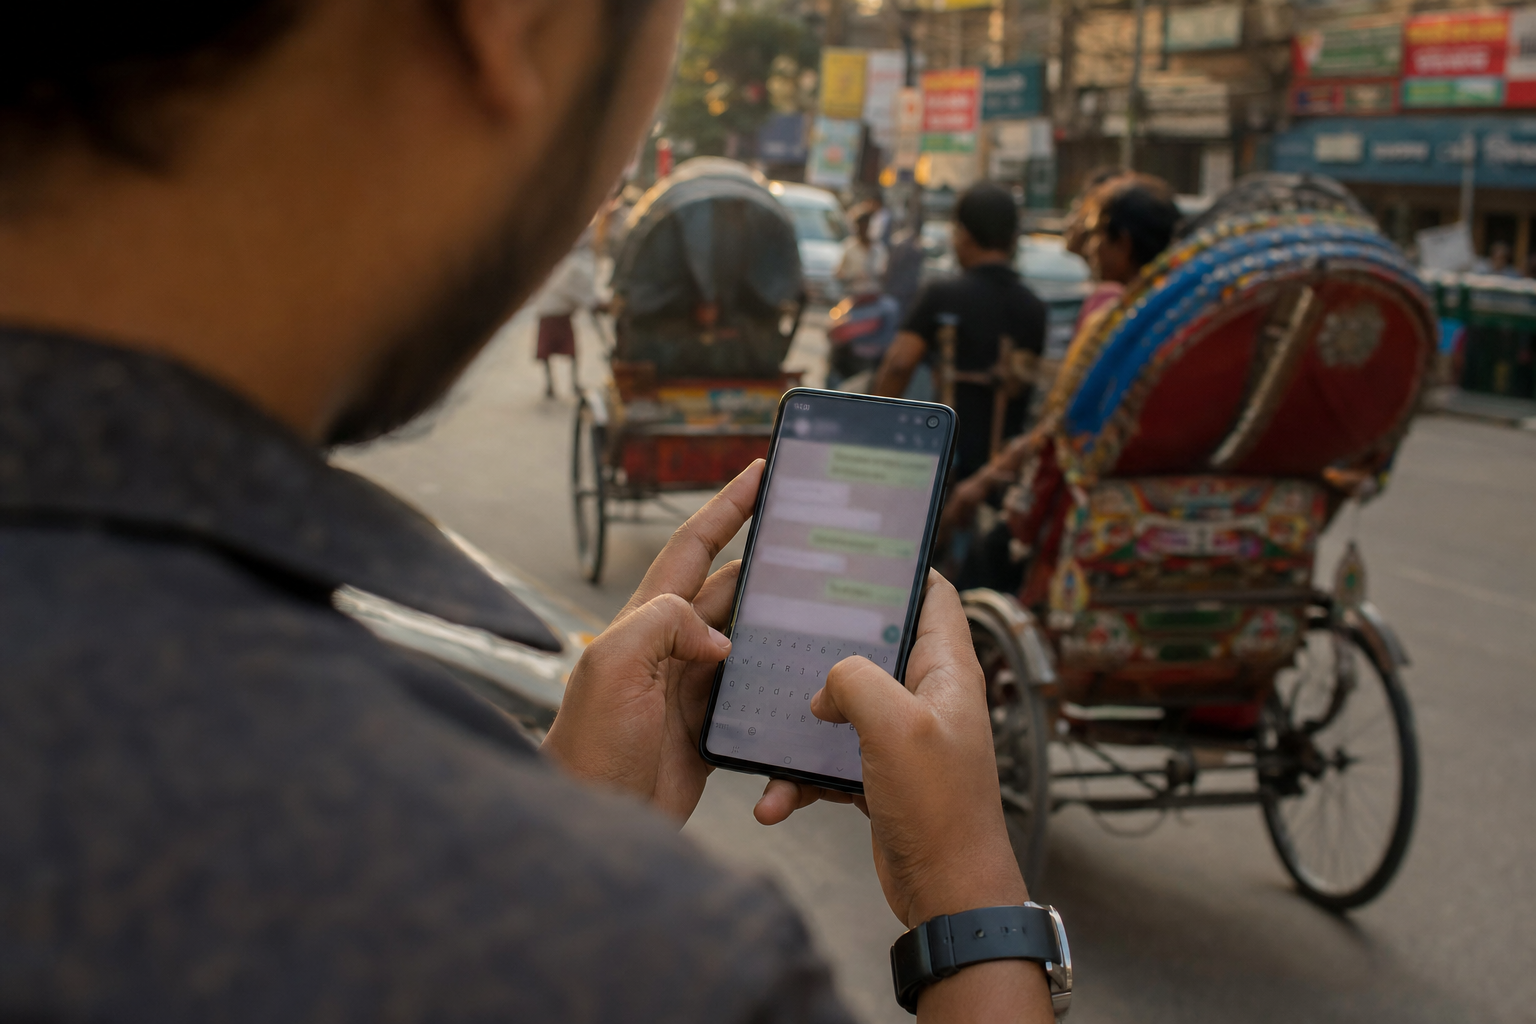
\includegraphics[width=6.5cm]{img/wild-typing.png}};
  \end{scope}
  \draw[rounded corners=10pt,rule,line width=0.8pt] (pc.south west) rectangle (pc.north east);
  % what they're typing: crisp Banglish bubbles over the photo
  \node[anchor=north west,fill=msggray,text=ink,rounded corners=6pt,inner sep=4pt,
        text width=2.6cm,font=\tiny\itshape,opacity=0.96,text opacity=1]
     at ([xshift=0.25cm,yshift=-0.25cm]pc.north west)
     {tomar final porikkha kemon holo?};
  \node[anchor=south west,fill=msgblue,text=white,rounded corners=6pt,inner sep=4pt,
        text width=2.9cm,font=\tiny\itshape,opacity=0.96,text opacity=1]
     at ([xshift=0.25cm,yshift=0.30cm]pc.south west)
     {kichu kothin chhilo, tobe asha kori valo hobe};
  \node[anchor=south east,font=\tiny,text=white!85]
     at ([xshift=-0.18cm,yshift=0.07cm]pc.south east) {AI-generated illustration};
\end{tikzpicture}

% ---------------- right column: search + review cards ----------------
\column{0.54\textwidth}
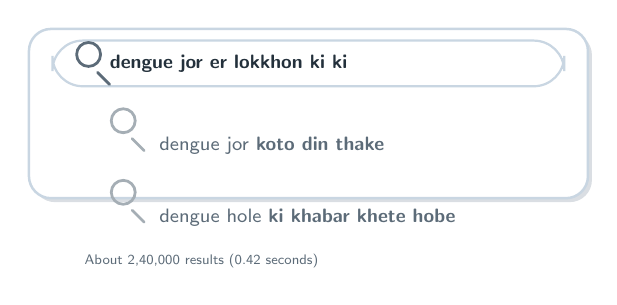
\begin{tikzpicture}[font=\scriptsize]
  \node[anchor=north west,draw=rule,fill=white,rounded corners=8pt,line width=0.9pt,
        minimum width=7.1cm,minimum height=2.15cm,
        drop shadow={shadow xshift=0.05cm,shadow yshift=-0.05cm,opacity=0.16,fill=buetnavy}]
        (sc) at (0,0) {};
  \node[anchor=north west,draw=rule,fill=white,rounded corners=11pt,line width=0.8pt,
        minimum width=6.5cm,minimum height=0.58cm] (bar)
     at ([xshift=0.3cm,yshift=-0.15cm]sc.north west) {};
  \node[anchor=west] at ([xshift=0.18cm]bar.west) {\ic{search}{subink}};
  \node[anchor=west,text=ink,font=\scriptsize\bfseries] at ([xshift=0.62cm]bar.west)
     {dengue jor er lokkhon ki ki};
  % autocomplete suggestions
  \node[anchor=north west,text=subink] (sg1) at ([xshift=0.62cm,yshift=-0.13cm]bar.south west)
     {\ic{search}{subink!55}\ \ dengue jor \textbf{koto din thake}};
  \node[anchor=north west,text=subink] (sg2) at ([yshift=-0.06cm]sg1.south west)
     {\ic{search}{subink!55}\ \ dengue hole \textbf{ki khabar khete hobe}};
  \node[anchor=north west,text=subink,font=\tiny] at ([xshift=-0.32cm,yshift=-0.10cm]sg2.south west)
     {About 2{,}40{,}000 results (0.42 seconds)};
\end{tikzpicture}

\vspace{0.14cm}

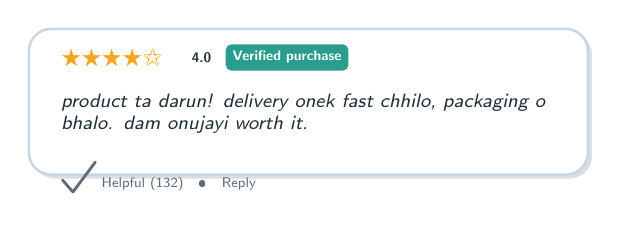
\begin{tikzpicture}[font=\scriptsize]
  \node[anchor=north west,draw=rule,fill=white,rounded corners=8pt,line width=0.9pt,
        minimum width=7.1cm,minimum height=1.85cm,
        drop shadow={shadow xshift=0.05cm,shadow yshift=-0.05cm,opacity=0.16,fill=buetnavy}]
        (rc) at (0,0) {};
  \node[anchor=north west,text=starorange,font=\small] (s)
     at ([xshift=0.3cm,yshift=-0.14cm]rc.north west)
     {\ding{72}\ding{72}\ding{72}\ding{72}\ding{73}};
  \node[anchor=west,font=\tiny\bfseries,text=ink] at ([xshift=0.12cm]s.east) {4.0};
  \node[anchor=west] at ([xshift=0.55cm]s.east) {\chip{good}{\tiny Verified purchase}};
  \node[anchor=north west,text=ink,text width=6.4cm,align=left] (rv)
     at ([yshift=-0.10cm]s.south west)
     {\textit{product ta darun! delivery onek fast chhilo, packaging o bhalo. dam onujayi worth it.}};
  \node[anchor=north west,text=subink,font=\tiny] at ([yshift=-0.10cm]rv.south west)
     {\ic{check}{subink}\ Helpful (132)\quad\textbullet\quad Reply};
\end{tikzpicture}

\end{columns}

\vspace{0.18cm}
\centering\small
Millions already type Bangla this way—\textbf{\color{accent}does the model stay as reliable when the input is Banglish?}
\end{frame}

% =====================================================  3. HIDDEN ACCESS GAP
\begin{frame}{The Hidden Access Gap\subt{Script as a controlled, measurable variable}}
\vspace{0.05cm}
\begin{columns}[T]
\begin{column}{0.5\textwidth}
\begin{keybox}
\centering\small
\textbf{If the task and gold answer are held fixed, does changing the script to Banglish change model reliability?}
\end{keybox}
\vspace{5pt}

\footnotesize
This is \emph{not} ``is Bangla hard for LLMs?''—already known. The missing piece is narrower:
\vspace{3pt}

\begin{itemize}\setlength\itemsep{2pt}
\item[\ic{globe}{accent}] \textbf{Script}, not language, is the variable.
\item[\ic{target}{accent}] Same item, same gold answer—\emph{did it flip?}
\item[\ic{ruler}{accent}] The gap is \textbf{measured}, not assumed.
\end{itemize}
\end{column}
\begin{column}{0.5\textwidth}
\centering
{\small\bfseries\color{ink} Same user, three doors to the model}\\[4pt]
\begin{tikzpicture}
  \node[rounded corners=9pt,fill=white,minimum width=6.4cm,minimum height=4.27cm,
        anchor=south west,
        drop shadow={shadow xshift=0.05cm,shadow yshift=-0.05cm,opacity=0.16,fill=buetnavy}]
        (dc) at (0,0) {};
  \begin{scope}
    \clip[rounded corners=9pt] (dc.south west) rectangle (dc.north east);
    \node[inner sep=0pt] at (dc.center) {
\includegraphics[width=6.4cm]{img/three-doors.png}};
  \end{scope}
  % script labels under each door, outcomes below
  \node[fill=cBangla,text=white,rounded corners=2.5pt,inner sep=3pt,font=\scriptsize\bfseries]
     at (1.33,1.00) {Bangla};
  \node[fill=cBanglish,text=white,rounded corners=2.5pt,inner sep=3pt,font=\scriptsize\bfseries]
     at (3.20,1.00) {Banglish};
  \node[fill=cEnglish,text=white,rounded corners=2.5pt,inner sep=3pt,font=\scriptsize\bfseries]
     at (5.07,1.00) {English};
  \node[text=good!70!white,font=\scriptsize] at (1.33,0.45) {\checkmark\ correct};
  \node[text=bad!55!white,font=\scriptsize\bfseries] at (3.20,0.45) {\ding{55}\ wrong};
  \node[text=good!70!white,font=\scriptsize] at (5.07,0.45) {\checkmark\ correct};
  \node[anchor=north east,font=\tiny,text=white!55]
     at ([xshift=-0.16cm,yshift=-0.08cm]dc.north east) {AI-generated};
\end{tikzpicture}
\end{column}
\end{columns}
\end{frame}

% =====================================================  4. RESEARCH QUESTION / FRAMING
\begin{frame}{Framing: Banglish as an Orthographic Access Problem}
\begin{keybox}
\normalsize\textbf{Central claim.} Script choice is a \emph{measurable robustness variable}: it can change accuracy, strict answer compliance, recoverability, and cost under controlled conditions.
\end{keybox}
\vspace{0.35cm}
\small Three design principles guide the whole study:
\vspace{0.15cm}

\begin{columns}[T]
\column{0.32\textwidth}
\featurecard{\linewidth}{accent}{\ic{target}{accent}}{1.\ \ Paired}{Same item id \& gold answer across all three scripts. Did \emph{this} item flip?}
\column{0.32\textwidth}
\featurecard{\linewidth}{cBangla}{\ic{doc}{cBangla}}{2.\ \ Audited}{Banglish is \emph{human-reviewed}, not raw machine transliteration. Rules out ``bad Banglish.''}
\column{0.32\textwidth}
\featurecard{\linewidth}{cBanglish}{\ic{scale}{cBanglish}}{3.\ \ Boundary}{Stronger models are a \emph{boundary test}, not a shortcut. Where does the gap end?}
\end{columns}
\vspace{0.2cm}
\centering\footnotesize\itshape\color{subink}
Not that Banglish is always harder—that reliability must be \emph{measured directly}, not assumed.
\end{frame}

% =====================================================  5. RELATED WORK
\begin{frame}{Related Work\subt{Three strands of prior work—and what each leaves open}}
\begin{columns}[T]
\column{0.5\textwidth}
\featurecard{\linewidth}{accent}{\ic{flask}{accent}}{Bengali task evaluation}{%
\textbf{BEnQA} (Shafayat et al., 2024) \textbullet\ \textbf{BanglaMATH} (Prama et al., 2025) \textbullet\ BnMMLU, BLUCK, BanglaQuAD, NCTB-QA \ldots\\[1pt]
{\color{subink}\itshape Active landscape—but script is never the controlled variable.}}\par\vspace{2pt}
\featurecard{\linewidth}{cBanglish}{\ic{chat}{cBanglish}}{Romanized \& code-mixed Bangla}{%
\textbf{BanglaTLit} (Fahim et al., 2024) \textbullet\ BanglishRev \textbullet\ BanTH \textbullet\ BnSentMix\\[1pt]
{\color{subink}\itshape Prevalence evidence—classification corpora, not paired QA.}}
\column{0.5\textwidth}
\featurecard{\linewidth}{cBangla}{\ic{bolt}{cBangla}}{Script robustness—nearest neighbors}{%
Translit.\ perturbations (Haider et al., 2025) \textbullet\ Script Gap (Khullar et al., 2025) \textbullet\ Romanized Nepali (Rimal \& Rimal, 2026)\\[1pt]
{\color{subink}\itshape No gold-answer QA/math; no reviewed romanization.}}\par\vspace{2pt}
\featurecard{\linewidth}{cEnglish}{\ic{ruler}{cEnglish}}{Tokenization \& latent language}{%
Tokenizer unfairness (Petrov et al., 2023) \textbullet\ latent English (Wendler et al., 2024) \textbullet\ RomanLens (2025)\\[1pt]
{\color{subink}\itshape Motivates our token \& oracle analyses—doesn't predict robustness.}}
\end{columns}
\vspace{0.16cm}
\centering\scriptsize\color{subink}
None of these measures whether the \textbf{same item, same gold answer} gets harder when only the \textbf{script} changes.
\end{frame}

% =====================================================  5b. GAP IN PRIOR WORK
\begin{frame}{Where We Sit\subt{Against the nearest neighbors, feature by feature}}
\footnotesize
Each nearest neighbor has one or two of the needed design elements—none has them together.
\vspace{0.08cm}

\centering
\renewcommand{\arraystretch}{1.05}
\scriptsize
\begin{tabular}{L{3.7cm} C{1.6cm} C{1.9cm} C{1.8cm} C{1.5cm} C{1.4cm}}
\toprule
\textbf{Work} & \textbf{Paired items} & \textbf{Human-rev.\ roman.} & \textbf{Downstream QA/math} & \textbf{Mitig.\ study} & \textbf{Scale ext.}\\
\midrule
Translit.\ perturbations {\color{subink}(Haider et al., 2025)} & \cpart & \cno & \cno & \cno & \cno\\
Script-gap triage {\color{subink}(Khullar et al., 2025)} & \cyes & \cno & \cno & \cno & \cno\\
Romanized Nepali {\color{subink}(Rimal \& Rimal, 2026)} & \cpart & \cno & \cno & \cyes & \cno\\
\rowcolor{accentlt}\textbf{\color{accent}This thesis} & \cyes & \cyes & \cyes & \cyes & \cyes\\
\bottomrule
\end{tabular}
\vspace{0.05cm}

{\centering\scriptsize\color{subink}\cyes\ covered \quad \cpart\ partial \quad \cno\ absent\par}
\vspace{0.05cm}

\begin{keybox}
\small We combine \textbf{all five} for the first time, under one protocol—the first paired, human-reviewed, multi-model Banglish robustness study with downstream QA/math and a scale extension.
\end{keybox}
\end{frame}

% =====================================================  6. CONTRIBUTIONS
\begin{frame}{Contributions\subt{Five, under one protocol}}
\vspace{0.05cm}
\begin{columns}[T]
\column{0.5\textwidth}
\featurecard{\linewidth}{accent}{\ic{target}{accent}}{1.\ \ Paired BN / BG / EN protocol}{Same QA \& math items in three script views; item id, answer type, and gold answer preserved.}\par\vspace{3pt}
\featurecard{\linewidth}{cBangla}{\ic{doc}{cBangla}}{2.\ \ Reviewed gold-core set}{200-item slice (144 BEnQA + 56 BanglaMATH); Banglish \emph{frozen} after targeted human review.}\par\vspace{3pt}
\featurecard{\linewidth}{cEnglish}{\ic{ruler}{cEnglish}}{3.\ \ Not cleanup or token length}{Review barely moves scores; Banglish is \emph{token-cheaper} than Bangla yet scores lower.}

\column{0.5\textwidth}
\featurecard{\linewidth}{cBanglish}{\ic{scale}{cBanglish}}{4.\ \ Frontier \& scale boundary}{5 hosted models + a \textbf{974-row gold extension} (1{,}174 paired items). Every model—incl.\ GPT-5.5—keeps a significant deficit at scale.}\par\vspace{3pt}
\featurecard{\linewidth}{bad}{\ic{gear}{bad}}{5.\ \ Negative mitigation evidence}{Self-normalization, generated views, and LoRA all fail to give a general fix—the weakness runs deep.}\par\vspace{4pt}
\begin{keybox}
\footnotesize\textbf{\color{accent}One-line thesis:} Banglish is an \textbf{undermeasured orthographic robustness challenge}—measure it, don't assume it.
\end{keybox}
\end{columns}
\end{frame}

% =====================================================  SECTION: BENCHMARK
\sectiondivider{Benchmark \& Protocol}{How we make \emph{script} the only variable}

% =====================================================  7. BENCHMARK PIPELINE
\begin{frame}{Benchmark Construction\subt{Two tracks, one paired protocol}}
\centering
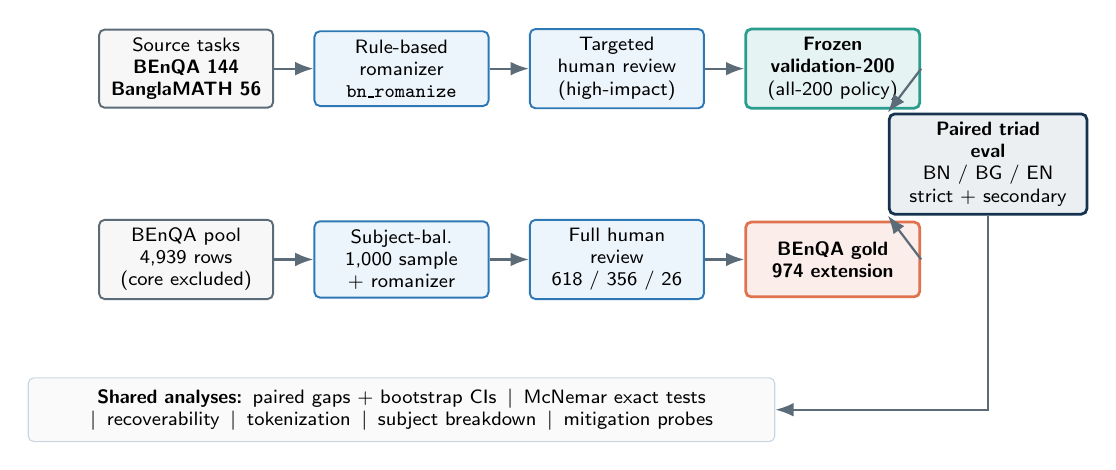
\begin{tikzpicture}[font=\scriptsize,
  box/.style={draw,rounded corners=2pt,minimum height=0.95cm,text width=2.0cm,align=center,inner sep=3pt,line width=0.7pt},
  src/.style={box,draw=subink,fill=gray!6},
  proc/.style={box,draw=accent,fill=accentlt},
  frozen/.style={box,draw=cBangla,fill=cBangla!12,line width=1pt},
  gold/.style={box,draw=cBanglish,fill=cBanglish!12,line width=1pt},
  ar/.style={-{Latex},line width=0.8pt,subink}]

% top track
\node[src] (s1) {Source tasks\\\textbf{BEnQA 144}\\\textbf{BanglaMATH 56}};
\node[proc,right=0.5cm of s1] (s2) {Rule-based\\romanizer\\\texttt{bn\_romanize}};
\node[proc,right=0.5cm of s2] (s3) {Targeted\\human review\\(high-impact)};
\node[frozen,right=0.5cm of s3] (s4) {\textbf{Frozen}\\\textbf{validation-200}\\(all-200 policy)};

% bottom track
\node[src,below=1.4cm of s1] (b1) {BEnQA pool\\4{,}939 rows\\(core excluded)};
\node[proc,right=0.5cm of b1] (b2) {Subject-bal.\\1{,}000 sample\\+ romanizer};
\node[proc,right=0.5cm of b2] (b3) {Full human\\review\\618 / 356 / 26};
\node[gold,right=0.5cm of b3] (b4) {\textbf{BEnQA gold}\\\textbf{974 extension}};

% evaluation hub
\node[box,draw=buetnavy,fill=buetnavy!8,line width=1pt,text width=2.3cm,right=0.7cm of $(s4)!0.5!(b4)$] (ev)
  {\textbf{Paired triad}\\\textbf{eval}\\BN / BG / EN\\strict + secondary};

\draw[ar] (s1)--(s2); \draw[ar] (s2)--(s3); \draw[ar] (s3)--(s4);
\draw[ar] (b1)--(b2); \draw[ar] (b2)--(b3); \draw[ar] (b3)--(b4);
\draw[ar] (s4.east) -- (ev.north west);
\draw[ar] (b4.east) -- (ev.south west);

% analyses bar
\node[draw=rule,fill=gray!4,rounded corners=2pt,below=1.0cm of b2,text width=9.2cm,align=center,inner sep=4pt] (an)
  {\textbf{Shared analyses:} paired gaps + bootstrap CIs \,\textbar\, McNemar exact tests \,\textbar\, recoverability \,\textbar\, tokenization \,\textbar\, subject breakdown \,\textbar\, mitigation probes};
\draw[ar] (ev.south) |- (an.east);
\end{tikzpicture}
\vspace{0.25cm}

\begin{columns}[T]
\column{0.5\textwidth}
\footnotesize\textbf{\color{cBangla}Validation-200 (core):} reviewed, mixed-task, frozen \emph{before} seeing outcomes.
\column{0.5\textwidth}
\footnotesize\textbf{\color{cBanglish}974 extension:} BEnQA-only, fully human-reviewed, for scale.
\end{columns}
\end{frame}

% =====================================================  8. EVALUATION PROTOCOL
\begin{frame}{Evaluation Protocol\subt{Models, scoring, and the paired gap}}
\begin{columns}[T]
\column{0.47\textwidth}
\featurecard{\linewidth}{cBangla}{\ic{flask}{cBangla}}{Open Qwen triad — reproducible baselines}{%
\mchip{Qwen2.5-3B}\ \mchip{Qwen2.5-7B (8-bit)}\\[4pt]
\mchip{Qwen3-4B}}
\par\vspace{6pt}
\featurecard{\linewidth}{accent}{\ic{globe}{accent}}{Frontier / API panel — boundary test}{%
\mchip{Gemini 3.5 Flash}\ \mchip{GPT-5.5 low}\\[4pt]
\mchip{Claude Sonnet 4.6}\ \mchip{DeepSeek V4 Flash}\\[4pt]
\mchip{Llama 3.3 70B (Groq)}}
\par\vspace{6pt}
\centering\scriptsize\color{subink}
8 models $\times$ 3 script views $\times$ paired items
\column{0.53\textwidth}
\footnotesize
\textbf{Scoring — two lenses}
\smallskip

\ic{target}{accent}\ \ \textbf{Strict} — deployable form, the contract.\\[4pt]
\ic{check}{good}\ \ \textbf{Secondary} — credit for recoverable answers (units, light markdown).
\medskip

\textbf{The paired gap} (per model, per item):
\begin{keybox}
\centering\footnotesize
$\Delta \,=\,$ {\color{cBanglish}\textbf{acc(reviewed Banglish)}} $\,-\,$ {\color{cBangla}\textbf{acc(Bangla)}}
\end{keybox}
\smallskip
\centering\scriptsize\color{subink}
Negative $\Rightarrow$ Banglish less accurate.\\
Paired bootstrap CIs + Holm-corrected \textbf{McNemar exact} tests.
\end{columns}
\end{frame}

% =====================================================  SECTION: RESULTS
\sectiondivider{Main Results}{Reviewed Banglish is consistently harder}

% =====================================================  9. MAIN RESULT TABLE
\begin{frame}{Main Result\subt{Validation-200, strict accuracy}}
\centering
\renewcommand{\arraystretch}{1.45}
\begin{tabular}{L{3.1cm} C{2.0cm} C{2.2cm} C{2.0cm} C{1.6cm} C{1.6cm}}
\toprule
\textbf{Model} & \textbf{\color{cBangla}Bangla} & \textbf{\color{cBanglish}Rev.\ Banglish} & \textbf{\color{cEnglish}English} & \textbf{BG $-$ BN} & \textbf{BG $-$ EN}\\
\midrule
Qwen2.5-3B      & \accbar{54}{200}{cBangla} & \accbar{41}{200}{cBanglish} & \accbar{71}{200}{cEnglish} & \gp{$-$6.5} & \gp{$-$15.0}\\
Qwen2.5-7B 8-bit & \accbar{65}{200}{cBangla} & \accbar{47}{200}{cBanglish} & \accbar{94}{200}{cEnglish} & \gp{$-$9.0} & \gp{$-$23.5}\\
Qwen3-4B        & \accbar{80}{200}{cBangla} & \accbar{49}{200}{cBanglish} & \accbar{88}{200}{cEnglish} & \gp{$-$15.5} & \gp{$-$19.5}\\
\bottomrule
\end{tabular}

{\scriptsize\color{subink} bars: items correct out of 200, strict scoring}
\vspace{0.4cm}

\begin{columns}[T]
\column{0.55\textwidth}
\begin{keybox}
\small For \textbf{every} Qwen model, reviewed Banglish is the \textbf{lowest} script view—below both native Bangla \emph{and} English.
\end{keybox}
\column{0.45\textwidth}
\footnotesize
$\bullet$ BG $-$ BN: \textbf{$-$6.5 to $-$15.5} pts\\[2pt]
$\bullet$ BG $-$ EN: \textbf{$-$15 to $-$23.5} pts — many failures are \emph{not} item difficulty: the same item is answerable in another view.
\end{columns}
\end{frame}

% =====================================================  10. MAIN RESULT CHART
\begin{frame}[fragile]{Main Result\subt{The pattern is visual and consistent}}
\centering
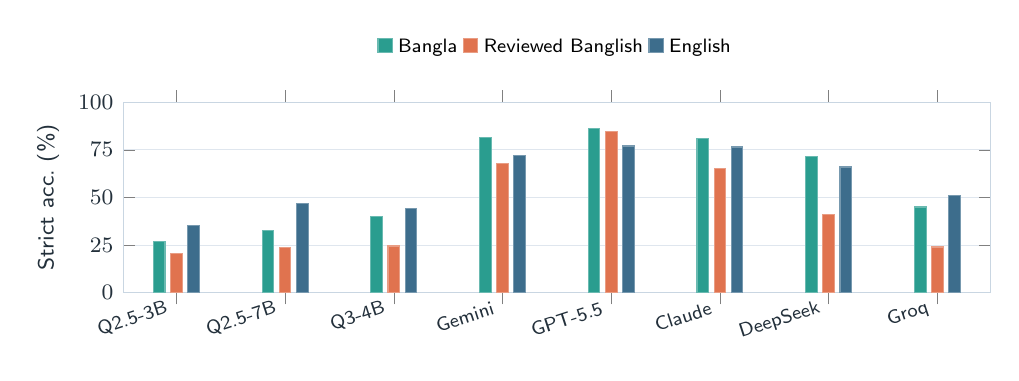
\begin{tikzpicture}
\begin{axis}[
  width=12.6cm, height=4.0cm,
  ybar, bar width=4.2pt,
  enlarge x limits=0.07,
  ymin=0, ymax=100,
  ylabel={Strict acc.\ (\%)},
  symbolic x coords={Q2.5-3B,Q2.5-7B,Q3-4B,Gemini,GPT-5.5,Claude,DeepSeek,Groq},
  xtick=data, x tick label style={font=\scriptsize,rotate=18,anchor=east},
  ytick={0,25,50,75,100}, ymajorgrids,
  legend style={font=\scriptsize,at={(0.5,1.18)},anchor=south,legend columns=3,draw=none},
  legend image code/.code={\draw[#1] (0cm,-0.06cm) rectangle (0.18cm,0.12cm);},
  nodes near coords style={font=\tiny},
]
\addplot[fill=cBangla,draw=cBangla!70] coordinates {(Q2.5-3B,27)(Q2.5-7B,32.5)(Q3-4B,40)(Gemini,81.5)(GPT-5.5,86)(Claude,81)(DeepSeek,71.5)(Groq,45)};
\addplot[fill=cBanglish,draw=cBanglish!70] coordinates {(Q2.5-3B,20.5)(Q2.5-7B,23.5)(Q3-4B,24.5)(Gemini,68)(GPT-5.5,84.5)(Claude,65)(DeepSeek,41)(Groq,24)};
\addplot[fill=cEnglish,draw=cEnglish!70] coordinates {(Q2.5-3B,35.5)(Q2.5-7B,47)(Q3-4B,44)(Gemini,72)(GPT-5.5,77)(Claude,76.5)(DeepSeek,66)(Groq,51)};
\legend{Bangla,Reviewed Banglish,English}
\end{axis}
\end{tikzpicture}

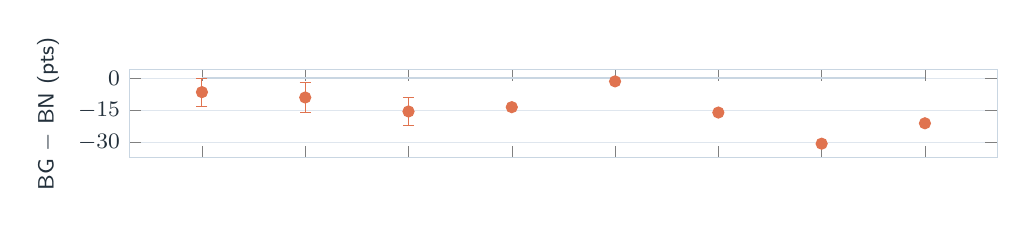
\begin{tikzpicture}
\begin{axis}[
  width=12.6cm, height=2.7cm,
  ymax=4, ymin=-37,
  ylabel={BG $-$ BN (pts)},
  symbolic x coords={Q2.5-3B,Q2.5-7B,Q3-4B,Gemini,GPT-5.5,Claude,DeepSeek,Groq},
  xtick=data, xticklabels={,,,,,,,},
  ytick={0,-15,-30}, ymajorgrids,
  scatter/classes={a={mark=*,cBanglish}},
]
\draw[rule,line width=0.6pt] (axis cs:Q2.5-3B,0) -- (axis cs:Groq,0);
% point estimates with CI error bars where available
\addplot[only marks,mark=*,cBanglish,mark size=2pt,
  error bars/.cd,y dir=both,y explicit]
 coordinates {
  (Q2.5-3B,-6.5)  +- (0,6.5)
  (Q2.5-7B,-9.0)  +- (0,7.0)
  (Q3-4B,-15.5)   +- (0,6.5)
  (Gemini,-13.5)  +- (0,0)
  (GPT-5.5,-1.5)  +- (0,0)
  (Claude,-16.0)  +- (0,0)
  (DeepSeek,-30.5)+- (0,0)
  (Groq,-21.0)    +- (0,0)
 };
\end{axis}
\end{tikzpicture}

{\scriptsize\color{subink} Lowest bar for every model \textbf{except GPT-5.5}; the BG$-$BN interval excludes zero for \textbf{7 of 8} models.}
\end{frame}

% =====================================================  11. McNEMAR SIGNIFICANCE
\begin{frame}{Is It Statistically Real?\subt{McNemar exact tests on discordant pairs}}
\small
The paired design is the textbook McNemar setting: only items where exactly one script is correct count. $b$ = Bangla-only correct, $c$ = Banglish-only correct.
\vspace{0.3cm}

\centering
\renewcommand{\arraystretch}{1.3}
\begin{tabular}{L{3.2cm} C{1.0cm} C{1.0cm} C{2.8cm} C{1.6cm} C{1.6cm}}
\toprule
\textbf{Model} & $b$ & $c$ & \textbf{Odds ratio [95\% CI]} & \textbf{Exact $p$} & \textbf{Holm $p$}\\
\midrule
Qwen2.5-3B      & 28 & 15 & 1.84 [0.99, 3.41] & 0.066 & 0.066\\
Qwen2.5-7B 8-bit & 37 & 19 & 1.92 [1.11, 3.32] & \gpp{0.022} & \gpp{0.044}\\
Qwen3-4B        & 39 & 8  & 4.65 [2.22, 9.75] & \gpp{$<$0.0001} & \gpp{$<$0.0001}\\
\bottomrule
\end{tabular}
\vspace{0.4cm}

\begin{keybox}
\small Qwen3-4B and Qwen2.5-7B stay significant after Holm correction. Qwen2.5-3B is marginal on the 200-core ($p=0.066$)—but on the \textbf{974-row extension} the same model becomes significant ($p=0.024$). The marginal result reflects \emph{sample size}, not absence of effect.
\end{keybox}
\end{frame}

% =====================================================  12. ROBUSTNESS BATTERY
\begin{frame}{The Gap Survives Every Robustness Check}
\small Could the gap be an artifact? We attacked it from five directions. It survived all of them.
\vspace{0.15cm}

\renewcommand{\arraystretch}{1.15}
\centering\footnotesize
\begin{tabular}{L{4.3cm} L{5.0cm} C{2.4cm}}
\toprule
\textbf{Objection} & \textbf{Test} & \textbf{Outcome}\\
\midrule
``Banglish is just bad'' & v5 targeted human review, then freeze & \chip{good}{$\leq$ 2 items}\\
``A few bad source rows'' & strict-197 (drop 3 flagged rows) & \chip{good}{still $-$7 to $-$16}\\
``It's the prompt wording'' & 2 neutral templates (terse, exam-role) & \chip{good}{$-$3 to $-$4.5}\\
``It's greedy decoding'' & temperature 0.7 & \chip{good}{$-$4.5}\\
``It's tokenization length'' & audited tokens-per-word & \chip{warn}{cheaper, not longer}\\
\bottomrule
\end{tabular}
\vspace{0.3cm}

\begin{keybox}
\footnotesize Review \emph{improves dataset quality} while preserving the central pattern. The gap stays negative under every template and temperature—the weakness is \textbf{script-conditioned}, not a wording or decoding accident.
\end{keybox}
\end{frame}

% =====================================================  13. TOKENIZATION
\begin{frame}[fragile]{Tokenization\subt{Cheaper but worse---cost and accuracy decouple}}
\begin{columns}[T]
\column{0.52\textwidth}
\centering
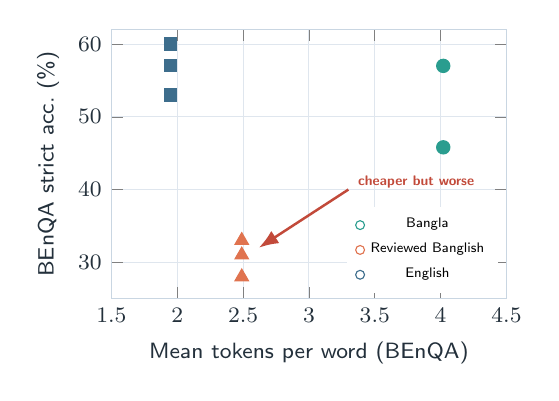
\begin{tikzpicture}
\begin{axis}[
  width=6.6cm,height=5.0cm,
  xlabel={Mean tokens per word (BEnQA)},
  ylabel={BEnQA strict acc.\ (\%)},
  xmin=1.5,xmax=4.5,ymin=25,ymax=62,
  xtick={1.5,2,2.5,3,3.5,4,4.5}, ymajorgrids, xmajorgrids,
  legend style={font=\tiny,at={(0.98,0.02)},anchor=south east,draw=none},
  legend image code/.code={\draw[#1] (0cm,0cm) circle (1.6pt);},
]
% Bangla points
\addplot[only marks,mark=*,cBangla,mark size=2.4pt] coordinates {(4.02,45.8)(4.02,57.0)(4.02,34.2)};
% Banglish
\addplot[only marks,mark=triangle*,cBanglish,mark size=2.8pt] coordinates {(2.49,28.0)(2.49,33.0)(2.49,31.0)};
% English
\addplot[only marks,mark=square*,cEnglish,mark size=2.2pt] coordinates {(1.95,57.0)(1.95,60.0)(1.95,53.0)};
\legend{Bangla,Reviewed Banglish,English}
\draw[-{Latex},bad,line width=0.9pt] (axis cs:3.3,40) -- (axis cs:2.62,32);
\node[bad,font=\tiny\bfseries,anchor=west] at (axis cs:3.3,41){cheaper \emph{but} worse};
\end{axis}
\end{tikzpicture}
\column{0.48\textwidth}
\footnotesize
\textbf{Mean tokens / word} (audited Qwen tokenizers):
\renewcommand{\arraystretch}{1.2}
\begin{tabular}{L{1.9cm} C{0.9cm} C{1.1cm} C{0.9cm}}
\toprule
& \color{cBangla}BN & \color{cBanglish}BG & \color{cEnglish}EN\\\midrule
BEnQA & 4.02 & \textbf{2.49} & 1.95\\
BanglaMATH & 4.63 & \textbf{2.11} & 1.41\\
\bottomrule
\end{tabular}
\medskip

\begin{keybox}
\small Reviewed Banglish uses \textbf{fewer} tokens per word than Bangla, yet scores \textbf{lower} for every model. It rules out the simple ``Banglish fails because it is longer'' story.
\end{keybox}
\smallskip
\scriptsize\color{subink} The failure is more consistent with script-conditioned lexical grounding than with context budget.
\end{columns}
\end{frame}

% =====================================================  14. SPELLING VARIATION
\begin{frame}{Spelling-Variation Robustness\subt{Not an artifact of one romanizer}}
\small
The clearest limitation of a rule-based romanizer: it is not natural, spelling-variable Banglish. So we generated \textbf{4 extra seeded respellings} per item (e.g.\ \texttt{sh\,$\to$\,s}, \texttt{bh\,$\to$\,v}) for 100 BEnQA items—5 spellings each.
\vspace{0.3cm}

\centering
\renewcommand{\arraystretch}{1.3}
\begin{tabular}{L{2.8cm} C{1.6cm} C{1.9cm} C{1.7cm} C{1.4cm}}
\toprule
\textbf{Model} & \textbf{Accuracy} & \textbf{Spelling range} & \textbf{Items flipping} & \textbf{Flip rate}\\
\midrule
Qwen2.5-3B & 31.2\% & 28--34\% & 17/100 & \textbf{17\%}\\
Qwen3-4B   & 29.0\% & 28--31\% & 6/100  & \textbf{6\%}\\
\bottomrule
\end{tabular}
\vspace{0.35cm}

\begin{columns}[T]
\column{0.5\textwidth}
\begin{takebox}{Magnitude is stable}
\small Accuracy stays in a narrow \textbf{28--34\%} band across independent spellings—the penalty is \emph{not} one romanizer's quirk.
\end{takebox}
\column{0.5\textwidth}
\begin{takebox}{Items are locally unstable}
\small Yet \textbf{17\%} of items flip correctness when only the spelling changes—same question, same answer.
\end{takebox}
\end{columns}
\end{frame}

% =====================================================  SECTION: WHY
\sectiondivider{Why Does It Fail?}{Recoverability and error taxonomy}

% =====================================================  15. RECOVERABILITY
\begin{frame}{Failure Analysis\subt{A large share of Banglish errors are recoverable}}
\small Paired item ids let us separate \emph{hard items} from \emph{script-specific failures}. Across 3 Qwen models $\times$ 200 items = 600 slots:
\vspace{0.25cm}

\centering
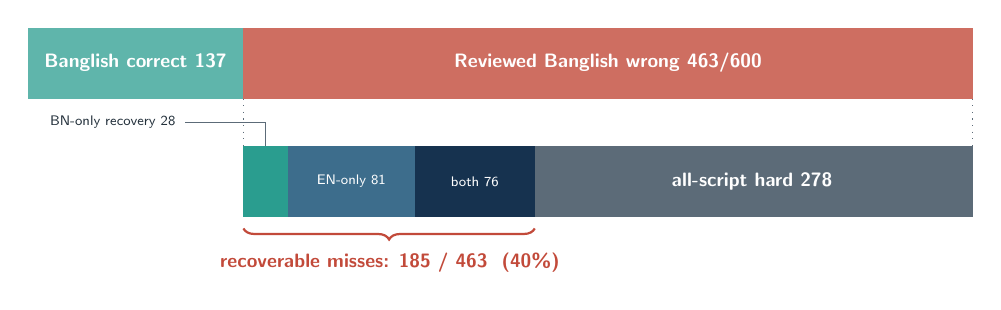
\begin{tikzpicture}[font=\scriptsize]
% top bar: correct vs wrong
\fill[cBangla!75] (0,1.6) rectangle (2.74,2.5);
\node[white,font=\scriptsize\bfseries] at (1.37,2.05){Banglish correct 137};
\fill[bad!80] (2.74,1.6) rectangle (12,2.5);
\node[white,font=\scriptsize\bfseries] at (7.37,2.05){Reviewed Banglish wrong \textbf{463/600}};

% decomposition of the 463
\fill[cBangla] (2.74,0.1) rectangle (3.30,1.0);   % bangla-only 28
\fill[cEnglish] (3.30,0.1) rectangle (4.92,1.0);  % english-only 81
\node[white,font=\tiny] at (4.11,0.55){EN-only 81};
\fill[buetnavy] (4.92,0.1) rectangle (6.44,1.0);  % both 76
\node[white,font=\tiny] at (5.68,0.55){both 76};
\fill[subink] (6.44,0.1) rectangle (12,1.0);      % all-script hard 278
\node[white,font=\scriptsize\bfseries] at (9.2,0.55){all-script hard 278};
% bangla-only label
\draw[subink,line width=0.4pt] (3.02,1.0) -- (3.02,1.3) -- (2.0,1.3);
\node[anchor=east,font=\tiny,text=ink] at (2.0,1.3){BN-only recovery 28};
% connectors
\draw[subink,dotted] (2.74,1.6) -- (2.74,1.0);
\draw[subink,dotted] (12,1.6) -- (12,1.0);
% bracket recoverable
\draw[decorate,decoration={brace,amplitude=4pt,mirror},bad,line width=0.8pt] (2.74,-0.05) -- (6.44,-0.05);
\node[bad,font=\scriptsize\bfseries,below=4pt] at (4.6,-0.1){recoverable misses: 185 / 463\ \ (40\%)};
\end{tikzpicture}
\vspace{0.25cm}

\begin{columns}[T]
\column{0.5\textwidth}
\begin{keybox}
\footnotesize \textbf{55\% of BEnQA Banglish misses are recoverable:} the same answer is reachable in Bangla or English.
\end{keybox}
\column{0.5\textwidth}
\footnotesize Yet \textbf{not absolute}: 20/600 slots are \emph{Banglish-only} wins. The claim is aggregate and paired—\emph{systematically} less reliable, not always worse.
\end{columns}
\end{frame}

% =====================================================  16. ERROR TAXONOMY
\begin{frame}[fragile]{Why Banglish Fails\subt{Error taxonomy of 164 recoverable misses}}
\begin{columns}[T]
\column{0.50\textwidth}
\footnotesize
\textbf{\color{subink}Taxonomy of recoverable BEnQA misses}
\vspace{0.18cm}

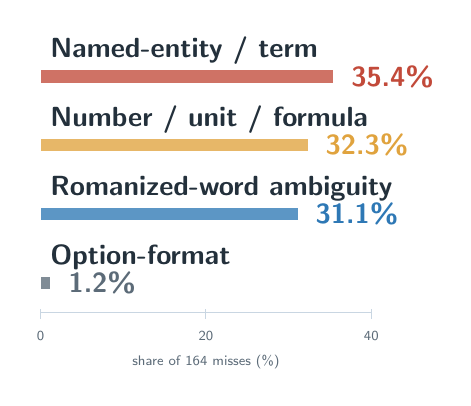
\begin{tikzpicture}[x=0.105cm,y=0.78cm,font=\scriptsize]
  \foreach \name/\val/\col/\yy in {
    {Named-entity / term}/35.4/bad/0,
    {Number / unit / formula}/32.3/warn/-1.12,
    {Romanized-word ambiguity}/31.1/accent/-2.24,
    {Option-format}/1.2/subink/-3.36} {
      \node[anchor=west,font=\bfseries,text=ink] at (0,\yy+0.52) {\name};
      \fill[\col!78] (0,\yy) rectangle (\val,{\yy+0.20});
      \node[anchor=west,font=\bfseries,text=\col] at ({\val+1.0},{\yy+0.10}) {\val\%};
  }
  \draw[rule,line width=0.4pt] (0,-3.74) -- (40,-3.74);
  \foreach \x in {0,20,40} {
    \draw[rule,line width=0.4pt] (\x,-3.69) -- (\x,-3.84);
    \node[anchor=north,text=subink,font=\tiny] at (\x,-3.89) {\x};
  }
  \node[anchor=north,text=subink,font=\tiny] at (20,-4.27) {share of 164 misses (\%)};
\end{tikzpicture}
\column{0.50\textwidth}
\begin{keybox}
\footnotesize \textbf{No single dominant failure mode.} A narrow parser, prompt, or spelling cleanup cannot close the gap by itself.
\end{keybox}
\vspace{0.18cm}

\scriptsize
\begin{itemize}\setlength\itemsep{2pt}\setlength\parskip{0pt}
\item \textbf{Technical terms become opaque:} \emph{lyakotik esid} $\to$ lactic acid.
\item \textbf{Numbers, units, formulas drift} in mixed numeric + romanized context.
\item \textbf{Latin spellings create ambiguity} for Bangla words and named entities.
\end{itemize}
\vspace{0.08cm}
{\scriptsize\color{subink}\textbf{Format is not the story:} option-format failures are only 1.2\%.}
\end{columns}
\end{frame}

% =====================================================  SECTION: FRONTIER
\sectiondivider{Frontier \& Scale}{Does capability or size fix it?}

% =====================================================  17. SCALING
\begin{frame}[fragile]{Within-Family Scaling\subt{The gap \emph{widens} with model size}}
\begin{columns}[T]
\column{0.56\textwidth}
\centering
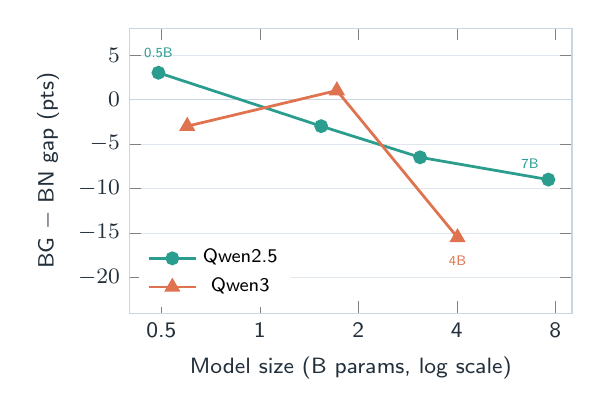
\begin{tikzpicture}
\begin{axis}[
  width=7.2cm,height=5.2cm,
  xmode=log, log basis x=10,
  xlabel={Model size (B params, log scale)},
  ylabel={BG $-$ BN gap (pts)},
  xmin=0.4,xmax=9, ymin=-24,ymax=8,
  xtick={0.5,1,2,4,8},
  xticklabels={0.5,1,2,4,8},
  ytick={5,0,-5,-10,-15,-20}, ymajorgrids,
  legend style={font=\scriptsize,at={(0.02,0.02)},anchor=south west,draw=none},
]
\draw[rule,line width=0.6pt] (axis cs:0.4,0) -- (axis cs:9,0);
\addplot[cBangla,mark=*,line width=1pt,mark size=2pt] coordinates {(0.49,3.0)(1.54,-3.0)(3.09,-6.5)(7.62,-9.0)};
\addplot[cBanglish,mark=triangle*,line width=1pt,mark size=2.4pt] coordinates {(0.60,-3.0)(1.72,1.0)(4.02,-15.5)};
\legend{Qwen2.5,Qwen3}
\node[font=\tiny,cBangla,anchor=east] at (axis cs:7.62,-7.2){7B};
\node[font=\tiny,cBanglish,anchor=north] at (axis cs:4.02,-16.5){4B};
\node[font=\tiny,cBangla,anchor=south] at (axis cs:0.49,3.6){0.5B};
\end{axis}
\end{tikzpicture}
\column{0.44\textwidth}
\footnotesize
Qwen2.5 shows a \textbf{clean monotonic trend}: the gap moves $+3.0 \to -3.0 \to -6.5 \to -9.0$ as size grows, with McNemar $p$ falling $0.26 \to 0.02$.
\smallskip

Qwen3's largest model has \textbf{by far the biggest gap} ($-15.5$, $p<0.0001$).
\medskip

\begin{keybox}
\small Added capability is preferentially spent on the higher-resource Bangla and English views. The script gap is \textbf{not something scaling alone fixes}—within these families it grows.
\end{keybox}
\end{columns}
\end{frame}

% =====================================================  18. FRONTIER + 974 EXTENSION
\begin{frame}{Frontier \& Scale Boundary\subt{The strongest result}}
\footnotesize
GPT-5.5 \emph{nearly closes} the gap on the 200-core (secondary scoring). But scale tells the real story: a 974-row human-reviewed gold extension.
\vspace{0.12cm}

\centering
\renewcommand{\arraystretch}{1.05}
\begin{tabular}{L{2.9cm} C{1.0cm} C{1.4cm} C{1.0cm} C{1.4cm} C{2.0cm} C{1.3cm}}
\toprule
\textbf{Model (974-row)} & \textbf{\color{cBangla}BN} & \textbf{\color{cBanglish}Banglish} & \textbf{\color{cEnglish}EN} & \textbf{BG$-$BN} & \textbf{95\% CI} & \textbf{McN.\ $p$}\\
\midrule
Qwen2.5-3B       & 33.2 & 29.3 & 50.3 & \gp{$-$3.9}  & [$-$7.2,\,$-$0.5] & 0.024\\
Gemini 3.5 Flash & 76.3 & 65.0 & 69.8 & \gp{$-$11.3} & [$-$13.7,\,$-$8.9] & $<$.0001\\
GPT-5.5 (none)   & 84.2 & 71.8 & 84.7 & \gp{$-$12.4} & [$-$15.1,\,$-$9.8] & $<$.0001\\
Claude Sonnet 4.6 & 78.4 & 53.8 & 79.2 & \gp{$-$25.4} & [$-$28.6,\,$-$21.9] & $<$.0001\\
DeepSeek V4 Flash & 77.6 & 45.0 & 81.2 & \gp{$-$32.7} & [$-$36.0,\,$-$29.3] & $<$.0001\\
Groq Llama 3.3 70B & 56.2 & 34.2 & 63.9 & \gp{$-$22.0} & [$-$25.7,\,$-$18.2] & $<$.0001\\
\bottomrule
\end{tabular}
\vspace{0.18cm}

\noindent
\statcard{3.05cm}{bad}{6 / 6}{models keep a significant deficit at scale}\hfill
\statcard{3.05cm}{cBanglish}{$-$12.4}{GPT-5.5 still fails (pts, $p\!<\!.0001$)}\hfill
\statcard{3.05cm}{bad}{$-$32.7}{DeepSeek—worst, despite high BN/EN}\hfill
\statcard{3.05cm}{accent}{1{,}174}{paired items (200 core $+$ 974 gold)}
\vspace{0.08cm}

{\centering\footnotesize\color{subink} GPT-5.5's near-closure on 200 items does \emph{not} generalize—\textbf{high absolute accuracy $\neq$ Banglish robustness.}\par}
\end{frame}

% =====================================================  SECTION: MITIGATION
\sectiondivider{Mitigation}{What if we try to fix it?}

% =====================================================  19. MITIGATION
\begin{frame}{Mitigation Attempts\subt{An honest negative result}}
\small We tried the natural fixes on \emph{both} sides of the model. None gives a general, deployable solution.
\vspace{0.12cm}

\renewcommand{\arraystretch}{1.15}
\centering
\begin{tabular}{L{4.1cm} L{5.2cm} C{2.6cm}}
\toprule
\textbf{Approach} & \textbf{Finding} & \textbf{Verdict}\\
\midrule
Self-normalization & Helps Qwen2.5-3B (+6.5) but \emph{hurts} Qwen3-4B ($-$12.5) & \chip{bad}{model-dependent}\\
Generated alt-script views & Routing too sparse; views not reliable enough & \chip{bad}{brittle}\\
LoRA adapter (eval-disjoint) & Gap $-6.5 \to -5.5$ / $-4.0$; \emph{not} significant & \chip{warn}{slight, $p>0.3$}\\
\bottomrule
\end{tabular}
\vspace{0.18cm}

\begin{columns}[c]
\column{0.70\textwidth}
\begin{keybox}
\footnotesize Light, eval-disjoint LoRA—the natural first training-side fix—narrows the gap only slightly and \textbf{not reliably}. The weakness is \textbf{deeper than a small adapter can close}. \emph{A negative result is still useful.}
\end{keybox}
\column{0.28\textwidth}
\centering

\includegraphics[width=0.95\linewidth]{img/bandaid-crack-crop.png}\\[-2pt]
{\tiny\color{subink} AI-generated illustration}
\end{columns}
\end{frame}

% =====================================================  20. CONCLUSION
\begin{frame}{Conclusion}
\begin{columns}[T]
\column{0.54\textwidth}
\small\textbf{What we showed}
\begin{itemize}\setlength\itemsep{5pt}
\item[\ic{check}{good}] Script choice \textbf{changes reliability} under controlled conditions—surviving review, tokenization, scaling, and frontier comparison.
\item[\ic{check}{good}] The gap is \textbf{statistically significant} for every model at scale, including GPT-5.5.
\item[\ic{check}{good}] High absolute accuracy does \textbf{not} guarantee Banglish robustness.
\item[\ic{check}{good}] Naive mitigation is \textbf{brittle}; the weakness runs deep.
\end{itemize}
\column{0.46\textwidth}
\small\textbf{Why it matters}
\begin{takebox}{The practical lesson}
\small For Bangla users, Latin-script input is a \textbf{real access path}—not informal noise models will automatically handle.
\smallskip

Robust evaluation must \textbf{measure it directly}; robust mitigation must \textbf{preserve task, format, and script equivalence}.
\end{takebox}
\medskip
\footnotesize\color{subink} Banglish is an undermeasured orthographic robustness challenge for Bangla LLM use.
\end{columns}
\end{frame}

% =====================================================  21. QUESTIONS
{\setbeamertemplate{footline}{}
\begin{frame}[plain]
\begin{tikzpicture}[remember picture,overlay]
  \fill[buetnavy] (current page.south west) rectangle (current page.north east);
  \fill[accent] ([yshift=-1.35cm]current page.north west) rectangle ([yshift=-1.18cm]current page.north east);
  \node[anchor=north east] at ([xshift=-1.0cm,yshift=-0.42cm]current page.north east)
     {\buetbadge{1.05cm}};
  % students photo card, right side
  \node[rounded corners=10pt,fill=white,minimum width=5.7cm,minimum height=3.8cm,
        anchor=east,drop shadow={shadow xshift=0.06cm,shadow yshift=-0.06cm,opacity=0.35,fill=black}]
        (qpc) at ([xshift=-1.0cm,yshift=0.45cm]current page.east) {};
  \begin{scope}
    \clip[rounded corners=10pt] (qpc.south west) rectangle (qpc.north east);
    \node[inner sep=0pt] at (qpc.center) {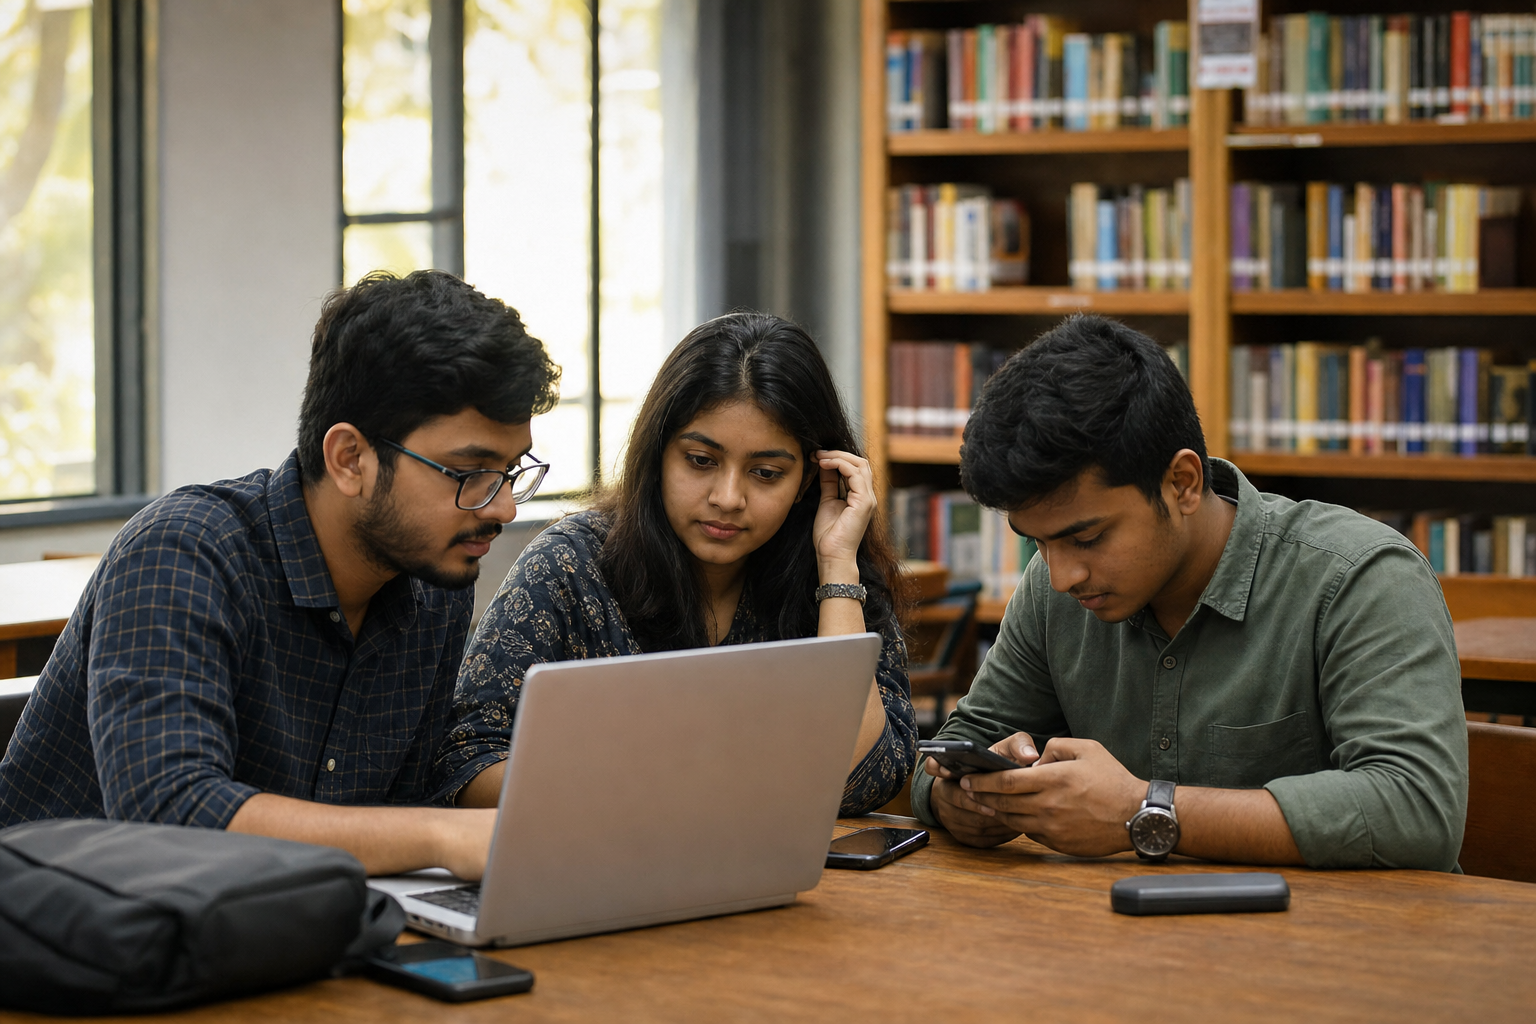
\includegraphics[width=5.7cm]{img/students.png}};
  \end{scope}
  \draw[rounded corners=10pt,white!30,line width=0.8pt] (qpc.south west) rectangle (qpc.north east);
  \node[anchor=north east,font=\tiny,text=white!45]
     at ([yshift=-0.06cm]qpc.south east) {AI-generated illustration};

  \node[anchor=west,text=white,font=\bfseries\fontsize{33}{37}\selectfont,text width=8.2cm]
     at ([xshift=1.0cm,yshift=1.55cm]current page.west) {Questions \&\\discussion};
  \node[anchor=west,text=accentlt,font=\fontsize{13}{17}\selectfont,text width=8.2cm]
     at ([xshift=1.05cm,yshift=-0.85cm]current page.west)
     {\textbf{Key takeaway:} Banglish robustness must be \mbox{measured} directly, not inferred from Bangla or English.};
  \node[anchor=south west,text=white!70,font=\footnotesize,text width=10.2cm]
     at ([xshift=1.0cm,yshift=0.8cm]current page.south west)
     {Munim Thahmid \textbullet\ 2005097 \quad\textbar\quad Supervisor: Dr.\ Sadia Sharmin};
  \node[anchor=south east,text=white!55,font=\scriptsize,align=right,text width=4.2cm]
     at ([xshift=-1.0cm,yshift=0.8cm]current page.south east)
     {BUET CSE\\B.Sc.\ Thesis Defense \textbullet\ June 2026};
\end{tikzpicture}
\end{frame}}

\end{document}
